\documentclass[11pt]{article}

\usepackage{nmrdoc}
\usepackage{siunitx}
\usepackage{bm}
\usepackage{tikz}

\sisetup{per-mode=symbol}
\DeclareSIUnit{\angstrom}{\text{\AA}}

\newcommand{\code}[1]{\texttt{#1}}
\setlength{\parindent}{0pt}
\setlength{\parskip}{0.42em}
\emergencystretch=2em

\begin{document}
\NmrTitle{Numerical Addendum: PiQuadrupole Calculator}

The PiQuadrupole calculator is a cutoff sum of one closed-form kernel,
evaluated per atom--ring pair. The shared ring geometry supplies a centre, a
fitted normal, and a mean radius; the calculator uses those numbers to evaluate
Stone's pre-contracted quadrupole electric-field-gradient kernel at nearby
atoms. That kernel contains the arithmetic. Around it sit the radius query and filters, the ring-frame
bookkeeping, the raw accumulation, and the shared \(T_0/T_1/T_2\) projection. The listings
below are distilled from the source: loops and bookkeeping are trimmed, but the
constants, guards, inequalities, tensor entries, and output shapes are the
implementation's.

\section{Ring geometry and pair gates}

\code{Protein::RingCount()} is the aromatic-ring count, so this calculator's
ring loop covers PHE, TYR, TRP6, TRP5, TRP9, HIS, HID, and HIE. Proline's
saturated pyrrolidine ring lives behind the separate saturated-ring accessor
and does not enter this path. For each aromatic ring,
\code{conf.ring\_geometries} gives a centre \(\bm c\), a unit normal
\(\hat{\bm n}\), a mean radius \(R\), and the ordered vertices. The normal is
the same SVD total-least-squares plane normal described in the Haigh--Mallion
numerical addendum: the right singular vector of the centred vertex
coordinates with the least spread. PiQuadrupole consumes that result and does
not refit it. The sign disambiguation the geometry routine applies to the
normal does not change the quadrupole kernel or scalar, because every term of
the kernel is even in \(\hat{\bm n}\). It does fix the sign convention for the
ring-neighbour \(z\) coordinate.

\begin{codebox}
// Distilled from GeometryResult.cpp and Ring.cpp.
conf.ring_geometries[ri] =
    protein.RingAt(ri).ComputeGeometry(positions);

geo.center = mean(geo.vertices);

Eigen::MatrixXd coords(geo.vertices.size(), 3);
for (size_t i = 0; i < geo.vertices.size(); ++i)
    coords.row(i) = (geo.vertices[i] - geo.center).transpose();

Eigen::JacobiSVD<Eigen::MatrixXd> svd(coords, Eigen::ComputeFullV);
geo.normal = svd.matrixV().col(2);       // least spread

Vec3 e1 = geo.vertices[1] - geo.vertices[0];
Vec3 e2 = geo.vertices[2] - geo.vertices[0];
if (geo.normal.dot(e1.cross(e2)) < 0) geo.normal = -geo.normal;

geo.radius = mean(norm(vertex - geo.center));
\end{codebox}

The spatial index builds a KD-tree over those ring centres. For an atom at
\(\bm r_i\), the radius query returns a candidate ring only when the squared
centre distance is strictly less than \code{ring\_current\_spatial\_cutoff}
squared. With \code{ring\_current\_spatial\_cutoff} set to
\(\SI{15.0}{\angstrom}\) in \code{data/calculator\_params.toml}, a ring centre
exactly \(\SI{15.0}{\angstrom}\) away is not proposed on the per-atom path.
This query only proposes pairs. The
closed-form kernel helper is called next, then the filter set decides whether
the pair changes any accumulator.

\begin{codebox}
// Distilled from PiQuadrupoleResult::Compute.
auto nearby_rings =
    spatial.RingsWithinRadius(atom_pos,
        cfg("ring_current_spatial_cutoff"));       // 15.0 A

PiQuadKernelResult kernel =
    ComputePiQuadKernel(atom_pos, geom.center, geom.normal);

KernelEvaluationContext ctx;
ctx.distance = kernel.distance;
ctx.source_extent = 2.0 * geom.radius;             // ring diameter
ctx.atom_index = ai;
ctx.source_ring_index = ri;

if (!filters.AcceptAll(ctx)) continue;
\end{codebox}

The helper itself returns a zero-initialized result when
\(r<\SI{0.1}{\angstrom}\), leaving \code{kernel.distance} at zero. The later
\code{MinDistanceFilter} requires \(r\ge\SI{0.1}{\angstrom}\), so that guarded
helper result becomes an omitted pair. At exactly
\(\SI{0.1}{\angstrom}\), the helper evaluates the inverse powers and the
minimum-distance filter accepts, subject to the later filters.

\code{DipolarNearFieldFilter} receives the ring diameter as
\code{source\_extent}. With the configured ratio \(0.5\), the per-atom path
accepts only
\[
  r > 0.5(2R)=R .
\]
Equality at the mean radius is rejected on this path. The
\code{RingBondedExclusionFilter} then removes ring vertices and atoms
covalently bonded to a ring vertex. A rejected pair is omitted from this
calculator's bookkeeping: it
does not create or update a ring-neighbour record, does not add the scalar
side channel, and does not add \(\bm G\) to the atom total.

The grid sampler follows the same kernel formula without atom topology. It
does not query the ring KD-tree; it loops over all aromatic rings and applies
three geometry tests. The grid path keeps equality at the mean radius and at
the \(\SI{15.0}{\angstrom}\) cutoff, and also at the singularity guard, because
its tests are strict on the skipped side.

\begin{codebox}
// Distilled from SampleKernelAt.
for (size_t ri = 0; ri < protein.RingCount(); ++ri) {
    const RingGeometry& geom = conf_->ring_geometries[ri];
    double r = (point - geom.center).norm();

    if (r < cfg("singularity_guard_distance")) continue;
    if (r < geom.radius) continue;
    if (r > cfg("ring_current_spatial_cutoff")) continue;

    auto kernel = ComputePiQuadKernel(point, geom.center, geom.normal);
    G_total += kernel.G;
}
\end{codebox}

\section{The pre-contracted kernel}

For an accepted pair, \code{d} is
\(\bm d=\bm r_i-\bm c\), the displacement from ring centre to atom, and
\(r=|\bm d|\). \code{ring\_normal} is the fitted unit vector
\(\hat{\bm n}\). The signed height is
\[
  h = \bm d\cdot\hat{\bm n},
\]
stored as \code{d\_dot\_n}. The helper also stores
\(\hat{\bm d}=\bm d/r\) as \code{result.direction}; that direction is later
copied into a newly created ring-neighbour record, but it is not used inside
the tensor formula.

\begin{figure}[ht]
\centering
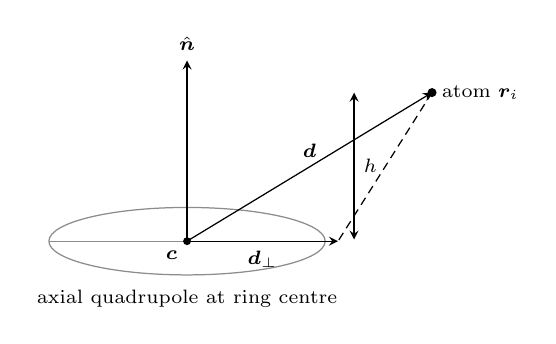
\begin{tikzpicture}[scale=1.02,line width=0.45pt,>=stealth]
  \coordinate (C) at (0,0);
  \coordinate (A) at (3.05,1.85);
  \coordinate (P) at (1.88,0.00);

  \draw[black!45] (C) ellipse (1.72 and 0.42);
  \draw[black!45] (-1.72,0) -- (1.72,0);
  \draw[->] (C) -- (0,2.25) node[above] {\scriptsize \(\hat{\bm n}\)};
  \draw[->] (C) -- (A) node[midway,above] {\scriptsize \(\bm d\)};
  \draw[densely dashed] (A) -- (P);
  \draw[->] (C) -- (P) node[midway,below] {\scriptsize \(\bm d_\perp\)};
  \draw[<->] (2.08,0.02) -- (2.08,1.85)
      node[midway,right] {\scriptsize \(h\)};

  \fill (C) circle (1.4pt) node[below left] {\scriptsize \(\bm c\)};
  \fill (A) circle (1.6pt) node[right] {\scriptsize atom \(\bm r_i\)};
  \node[below] at (0,-0.48) {\scriptsize axial quadrupole at ring centre};
\end{tikzpicture}
\caption{The code evaluates a point axial quadrupole at the fitted ring centre.
The closed form uses the centre-to-atom displacement \(\bm d\), the fitted
normal \(\hat{\bm n}\), and the height \(h=\bm d\cdot\hat{\bm n}\).}
\end{figure}

The rank-4 interaction tensor before contraction is the fourth derivative of
\(1/r\):
\[
\begin{aligned}
T_{abcd}={}&
  \frac{105\,d_a d_b d_c d_d}{r^9} \\
&-\frac{15}{r^7}\bigl(
  \delta_{ab}d_c d_d+\delta_{ac}d_b d_d+\delta_{ad}d_b d_c
 +\delta_{bc}d_a d_d+\delta_{bd}d_a d_c+\delta_{cd}d_a d_b\bigr)\\
&+\frac{3}{r^5}\bigl(
  \delta_{ab}\delta_{cd}
 +\delta_{ac}\delta_{bd}
 +\delta_{ad}\delta_{bc}\bigr).
\end{aligned}
\]
The code never stores this \(3^4\)-component object and never loops over
\(c,d\). The contraction with the source axis is done on paper:
\[
  G_{ab}=T_{abcd}\hat n_c\hat n_d .
\]
The products \(d_c d_d\hat n_c\hat n_d\) become \(h^2\), the
\(\delta_{cd}\) contraction becomes \(\hat{\bm n}\cdot\hat{\bm n}=1\), and
the four mixed Kronecker terms pair up as
\(-30h(\hat n_a d_b+\hat n_b d_a)/r^7\). That accounting is exactly the
five-term expression the helper evaluates.

\begin{codebox}
// Distilled from ComputePiQuadKernel.
Vec3 d = atom_pos - ring_center;
double r = d.norm();

if (r < cfg("singularity_guard_distance")) return result;  // zero

result.distance = r;
result.direction = d / r;

double r2 = r * r;
double r5 = r2 * r2 * r;
double r7 = r5 * r2;
double r9 = r7 * r2;

double h = d.dot(ring_normal);
double h2 = h * h;
double cos_theta = h / r;

result.scalar = (3.0*cos_theta*cos_theta - 1.0) / (r2*r2);

double delta_term = 3.0/r5 - 15.0*h2/r7;

for (int a = 0; a < 3; ++a) {
    for (int b = 0; b < 3; ++b) {
        double nd = ring_normal(a)*d(b) + ring_normal(b)*d(a);
        result.G(a,b) =
              105.0*h2*d(a)*d(b)/r9
            -  30.0*h*nd/r7
            -  15.0*d(a)*d(b)/r7
            +   6.0*ring_normal(a)*ring_normal(b)/r5
            + (a == b ? delta_term : 0.0);
    }
}
\end{codebox}

The denominator powers are built once as \(r^5\), \(r^7\), and \(r^9\).
The \(r^{-9}\) term carries \(h^2d_ad_b\), four powers of length;
the \(r^{-7}\) terms carry two powers of length; and the \(r^{-5}\) terms
carry none. Each completed tensor entry therefore has units
\(\si{\angstrom^{-5}}\), and \(r^{-5}\) is the kernel's far-field scale: the
length factors in the numerator cancel the higher explicit powers down to it.

The scalar side channel uses the same \(h\) and \(r\):
\[
  q = \frac{3(h/r)^2-1}{r^4}.
\]
Per accepted ring, \code{quad\_scalar} stores it. It is also accumulated by
aromatic ring type into \code{pq\_per\_type\_T0\allowbreak.npy}. That array
name contains \(T0\), but the number is not the trace component of \(\bm G\);
it is the separate Buckingham-style scalar kernel with units
\(\si{\angstrom^{-4}}\).

\section{Trace and accumulation}

The closed form is symmetric term by term. It is also traceless by the same
Laplace identity that removes the \(\delta_{cd}\) part of the physical axial
quadrupole contraction. Taking the trace of the code's expression gives
\[
  (105-60-45)\frac{h^2}{r^7}
  +(-15+6+9)\frac{1}{r^5}=0 .
\]
That cancellation uses \(\hat{\bm n}\cdot\hat{\bm n}=1\) and
\(\bm d\cdot\bm d=r^2\). The field point is away from the point-source
singularity after the guard, so the Laplace cancellation is the analytic
reason the kernel is pure \(T_2\).

The code does not apply a separate numerical de-tracing step to \code{G} or to
\code{G\_total}. There is no projection of the form
\(\bm G\leftarrow\bm G-\operatorname{tr}(\bm G)\bm I/3\) before storage. The
raw matrix is passed to \code{SphericalTensor::Decompose}; that routine records
the trace residue in \(T_0\) and subtracts the same trace only while forming
the stored \(T_2\) vector. Thus a floating-point trace residue is retained in
the packed nine-number output rather than forced to zero.

\begin{codebox}
// Distilled from the accepted-pair path in Compute.
if (!rn) {
    RingNeighbourhood new_rn;
    new_rn.ring_index = ri;
    new_rn.ring_type = ring.type_index;
    new_rn.distance_to_center = kernel.distance;
    new_rn.direction_to_center = kernel.direction;

    Vec3 d_vec = atom_pos - geom.center;
    double z = d_vec.dot(geom.normal);
    Vec3 d_plane = d_vec - z * geom.normal;
    new_rn.z = z;
    new_rn.rho = d_plane.norm();
    new_rn.theta = std::atan2(new_rn.rho, std::abs(z));

    conf_atom.ring_neighbours.push_back(new_rn);
    rn = &conf_atom.ring_neighbours.back();
}

rn->quad_tensor = kernel.G;
rn->quad_spherical = SphericalTensor::Decompose(kernel.G);
rn->quad_scalar = kernel.scalar;

int t = ring.TypeIndexAsInt();
if (t >= 0 && t < kAromaticRingTypeCount) {
    conf_atom.per_type_pq_scalar_sum[t] += kernel.scalar;
    for (int c = 0; c < 5; ++c)
        conf_atom.per_type_pq_T2_sum[t][c] += rn->quad_spherical.T2[c];
}

G_total += kernel.G;
\end{codebox}

The ring-frame record splits the same centre-to-atom vector into signed height
\(z\), in-plane radius \(\rho\), and folded polar angle
\(\operatorname{atan2}(\rho,|z|)\). The fold gives the same stored angle to
points mirrored across the fitted plane; the signed \(z\) keeps the face
orientation. These coordinates are bookkeeping for shared ring-neighbour
outputs. They do not feed back into the quadrupole formula, which has already
used \(h=\bm d\cdot\hat{\bm n}\).

The atom total is the raw sum of accepted per-ring matrices,
\[
  \bm G_i^{\mathrm{tot}} =
  \sum_{\rho\in\mathcal A_i}\bm G^{(i\rho)} ,
\]
where \(\mathcal A_i\) is the accepted aromatic-ring set for atom \(i\). The
calculator then decomposes that raw total.

\begin{codebox}
conf_atom.piquad_shielding_contribution =
    SphericalTensor::Decompose(G_total);

pq_shielding.npy     // N x 9:  [T0, T1[0..2], T2[0..4]]
pq_per_type_T0.npy   // N x 8:  scalar q sums by aromatic ring type
pq_per_type_T2.npy   // N x 40: 8 aromatic ring types x 5 T2 entries
\end{codebox}

Despite the \code{pq\_shielding.npy} filename, this array stores the unscaled
quadrupole EFG kernel in \(\si{\angstrom^{-5}}\). The code multiplies in neither
of the two physical factors this kernel would carry once calibrated: the
quadrupole strength \(\Theta\) and the Buckingham response coefficient (the
per-nucleus susceptibility that turns an electric-field gradient at the nucleus
into a shielding contribution). Both are outside \code{PiQuadrupoleResult}.

\section{The shared tensor projection}

\code{SphericalTensor::Decompose} is closed-form arithmetic on a \(3\times3\)
matrix \(\bm X\). The trace average gives \(T_0\), the antisymmetric part gives
the three \(T_1\) components, and the symmetric traceless part gives the five
\(T_2\) numbers. It does not diagonalize the matrix and does not extract
principal axes.

\begin{codebox}
st.T0 = sigma.trace() / 3.0;

st.T1[0] = 0.5*(sigma(1,2) - sigma(2,1));
st.T1[1] = 0.5*(sigma(2,0) - sigma(0,2));
st.T1[2] = 0.5*(sigma(0,1) - sigma(1,0));

double Sxx = sigma(0,0) - st.T0;
double Syy = sigma(1,1) - st.T0;
double Szz = sigma(2,2) - st.T0;
double Sxy = 0.5*(sigma(0,1) + sigma(1,0));
double Sxz = 0.5*(sigma(0,2) + sigma(2,0));
double Syz = 0.5*(sigma(1,2) + sigma(2,1));

st.T2[0] = std::sqrt(2.0) * Sxy;
st.T2[1] = std::sqrt(2.0) * Syz;
st.T2[2] = std::sqrt(3.0/2.0) * Szz;
st.T2[3] = std::sqrt(2.0) * Sxz;
st.T2[4] = (Sxx - Syy) / std::sqrt(2.0);
\end{codebox}

The \(T_2\) factors make the five-vector length equal to the Frobenius length
of the symmetric traceless matrix \(\bm S\). Each off-diagonal entry appears
twice in \(\bm S\), so \(\sqrt2\,S_{xy}\) squares to the two-entry
contribution \(2S_{xy}^2\). The two diagonal entries
\(\sqrt{3/2}\,S_{zz}\) and \((S_{xx}-S_{yy})/\sqrt2\) carry the remaining
diagonal degrees of freedom after the trace is removed. For PiQuadrupole, the
analytic tensor is symmetric and traceless, so it contributes only to
\(T_2\). The code still emits the shared nine-number packet and leaves any
computed \(T_0\) or \(T_1\) residue in place.

\section{Glossary}

\textbf{Stone rank-4 interaction tensor.} The fine grain of how a point
source's field bends in space (the fourth derivative of \(1/r\): not how it
slopes or curves, but how that curvature changes twice more along every pair of
Cartesian directions). In this calculator the source axis contracts the last
two indices, turning the \(81\) possible components of \(T_{abcd}\) into the
nine entries of \(G_{ab}\). Formally,
\(T_{abcd}=\partial_a\partial_b\partial_c\partial_d(1/r)\), evaluated away
from the source.

\textbf{Pre-contracted quadrupole kernel.} The rank-4 sum collapsed along the
source axis on paper (the contraction done algebraically, leaving the program a
\(3\times3\) formula to read off rather than \(81\) components to contract at
run time). The term
\(105h^2d_ad_b/r^9\) is the contracted form of
\(105d_ad_bd_cd_d\hat n_c\hat n_d/r^9\). Formally, the stored geometric EFG
kernel is \(G_{ab}=T_{abcd}\hat n_c\hat n_d\), with no physical quadrupole
strength multiplied in.

\textbf{Analytic tracelessness.} The three diagonal curvatures balance before
the numbers reach a projection routine. In the implemented formula, the trace
has \(h^2/r^7\) coefficient \(105-60-45\) and \(1/r^5\) coefficient
\(-15+6+9\), both zero. Formally, outside the source,
\(\operatorname{tr}\bm G=G_{aa}=T_{aacd}\hat n_c\hat n_d
=\nabla^2\partial_c\partial_d(1/r)\,\hat n_c\hat n_d=0\).

\textbf{Near-field exclusion.} A blind spot drawn around the source, where the
point-quadrupole stand-in is switched off because a ring seen from inside its
own radius is no longer a point (a distance filter on the centre separation).
For a ring of mean radius \(R\), the per-atom path omits the pair unless the
centre distance is greater than \(R\); equality is outside the accepted set.
Formally, the filter is \(r>\rho_{\mathrm{nf}}E\), with
\(E=2R\) and \(\rho_{\mathrm{nf}}=0.5\).

\textbf{Spherical tensor split.} A \(3\times3\) tensor holds three kinds of
content that rotate without mixing --- an orientation-free size (the scalar
trace, \(T_0\)), an axial twist from its antisymmetric part (the three \(T_1\)
components), and a five-number traceless shape for the rest of the
direction-dependence (the five \(T_2\) components). For
PiQuadrupole the analytic kernel contributes to the five-number part; the
nine-number output keeps the shared layout used by calculators whose tensors
also have scalar or antisymmetric parts. Formally, it is the closed-form split
of a \(3\times3\) tensor's nine components into dimensions \(1+3+5\), with the
\(T_2\) basis normalized to preserve the Frobenius norm.

\end{document}
